% ---------------------------------------------------
% CHAPTER SUMMARY MESSAGE: < WRITE THIS BEFORE ANY EDITING>
% ---------------------------------------------------

Machine learning does not exist without software. There are a large variety of algorithms written in different programming languages and general software frameworks that combine many classes of methods into one package. The following sections focus on specific topics and challenges related to machine learning software design in HEP.

%\subsection{HEP Machine-Learning Software}
%The HEP community has developed a baseline with which any new machine-learning tools or methods can be compared with.

%We are able to keep up and in some cases improve over external tools on HEP benchmarks. Internally-developed tools have GPU-capable deep-learning libraries. On the other hand, not all external data-formats, options, model architectures and variants are currently fully supported.

\subsection{Software Methodology}
Presently, there are two machine learning software methodologies in high-energy physics. The first approach is to implement abstract ML algorithms in HEP-developed toolkits, such as the Toolkit for Multivariate Analysis (TMVA) in ROOT. This provides on site support to physicists and dedicated development for HEP data formats and applications. The second approach is to rely on externally developed software, of which there are many examples. This often requires tedious and repetitive work to adapt HEP data formats to external software, breaks analysis workflows and introduces difficulties in the analysis software development. Historically, a variety of approaches and competition among them has led to important breakthroughs in the field. On the other hand, having too many choices increases repetition and leads community segmentation and possible issues with reproducibility.
There is some convergence of the two approaches. Converters have been written for the reintegration of some externally trained models into HEP tools, like~\cite{lwtnn}. Complementarily, interfaces between HEP and external tools have also been developed.%  More effort is needed to extend these interconnecting efforts and integrate new useful tools when they become available.

\subsection{I/O and Programming Languages}\label{sec:software_IO}
The sheer amount of data accumulated by HEP experiments requires data access optimization because. Such I/O performance is very dependent on data formats. Moreover, support for reading data in different formats is required for certain use-cases.
%In particular, data streaming, locality and partitioning will impact training and cost of data processing.

Exploration of new file systems and methods to improve I/O limitations are important and the following R\&D studies should take place:
\begin{itemize}
 \item Explore new file systems to assess I/O limitations;
 \item Use alternative industry approaches such as Google BigQuery to explore various data access patterns;
 \item Explore parallel data processing platforms such as Apache Spark for ML training.
\end{itemize}

Although particle physics has been reliant on C++ over the past decade, the machine learning community has explored other programming languages, in particular the python-based ecosystem.

\subsection{Software Interfaces to Acceleration Hardware}\label{sec:software_proglang}
Modern machine learning software significantly benefits from the use of hardware accelerators such as GPUs. At the same time, ML users should not be hindered in their development of new applications by writing platform-dependent code. Various interfaces to different hardware architectures are needed in order to make efficient use of the available computing resources. The emergence of the Open Computing Language (OpenCL) allows programming of high-level interfaces that can run on various hardware platforms.

Machine learning tools often provide different sets of APIs to develop and train the models in one language, and various bindings to use trained models in other programming languages. This is a convenient model for many HEP applications, such as the trigger system, where (1) application latency puts stringent requirements on the software and hardware used and (2) the general purpose training platform might be different from the highly specific deployment platform.

\subsection{Parallelization and Interactivity}
Training ML algorithms takes a significant amount of time and parallelization at various levels is desired, such as the parallelization of the computations within a single model. Another type of parallelism is data parallelism that targets the processing phase of the training with data partitioning and model training using distributed workers. Frameworks like Apache Spark and ideas such as batch training offer promise in this area.

One often needs to produce many different machine learning models, for example while tuning hyper-parameters or performing k-fold cross-validation, and distribution of these algorithms is key to the reduction of the overall training time.
ML algorithm inference significantly benefits from parallelization as well. Although event selection in a particle physics trigger system is ``embarassingly parallel~\cite{embarrassingly}'', parallel processing frameworks are developed to reduce the memory footprint. Complex models might well be too big to reside once per CPU core in memory and need to be hosted in shared memory. At the same time the stringent latency requirements impose constraints on the type of algorithms that can be easily deployed.

The availability of interactive frameworks, for example Jupyter notebooks, allows for rapid prototype development and testing of ML tools. Such frameworks also ease the connection between the description of models and the data, providing straightforward means of visualizing models and data.
HEP has started to exploring interactive frameworks, such as the Service for Web Based Analysis (SWAN)~\cite{swan}. One of the challenges is availability of adequate hardware resources for these systems.

%\subsection{Brief History of HEP Machine-Learning Software}
%\label{sec:software_history}

%\begin{description}
%\item[1991 - 1998]
%	\begin{itemize}
%		\item C. Peterson and T. Rognvaldsson, An Introduction to Artificial Neural Networks, Lectures given at the 1991 CERN School of Computing, University of Lund preprint LU TP 91-23, September 1991.
%		\item Early Feed-forward NN’s B. Denby, Neural Computation 5 (1993) 505.
%		\item Kernel Density http://inspirehep.net/record/407093
%		\item Fisher discriminants \& H-matrix http://inspirehep.net/record/1234704
%	\end{itemize}
%	\item[1998-2005] Initial HEP Machine Learning Software development based on external algorithms lead to number of standalone packages (MultilayerPerceptron and others)
%	\item[2005-2010] Abundance of comparably-performing methods lead to a consolidation into software toolkits such as Toolkit for Multivariate Analysis (TMVA) and StatPatternRecognition (SPR).
%	\item[2008] SPR stops development and support, TMVA takes over
%	\item[2010-2014] Wide use of TMVA in HEP, full integration in ROOT and switch to maintenance mode
%	\item[2014-present] Upgrade/modernization of TMVA, wider use of externally developed tools deep learning revolution.
%\end{description}

\subsection{Internal and External ML tools}
%Contributors: Juan Pedro Araque, Nuno Filipe Castro, Thomas Keck, Stefan Wunsch, Igor Lakomov, Konstantin Skazytkin, Luke Kreczko, Przemysław Karpiński, Claire David, Hans Pabst, Attilio Picazio, Giles Strong, Gordon Watts, Lorenzo Moneta, Matthew Feickert, Mark Neubauer, Daniele Bonacorsi, Mauro Verzetti, Seth Moortgat, Sergei Gleyzer, Fernanda Psihas, Elias Coniavitis, Gilles Louppe, Kim Albertsson, Steven Schramm, Martin Erdmann

% In Section~\ref{sec:data_formats} we provide a high-level overview of existing HEP and ML data formats. Section~\ref{sec:ml_tools} investigates the present ML software landscape in HEP, while Section~\ref{sec:tool_roadmap} proposes a road-map towards a sustainable future HEP machine learning software landscape.

Internally developed ML software, such as the Toolkit for Multivariate Analysis (TMVA,~\cite{TMVA}), has been developed to apply a variety of machine learning algorithms to HEP challenges. Currently, many published HEP analyses with machine learning have made use of TMVA. There is also software developed in HEP, such as NeuroBayes~\cite{neurobayes,neurobayes2} and RuleFit, that have gained popularity outside of HEP.

At the same time, the ML landscape has evolved and many different ML tools have emerged and gained popularity. There are a growing number of published results based on externally developed tools. The latter, often developed directly by industry for specific applications, are constantly undergoing development, incorporating the latest algorithms from academia. Currently, both internal and external tools are used by the HEP community. TMVA has also undergone significant development in recent years.
In addition, there are smaller tools developed in the HEP community, extending either internal or external ML tools for specific use cases and applications within HEP experiments, such as \texttt{hep\_ml}~\cite{hep_ml} for training ML classifiers, or \texttt{tmva-branch-adder}~\cite{tmva-branch-adder} and \texttt{lwtnn}~\cite{lwtnn} to facilitate classifier inference tasks.

This begs the question: what aspects of ML development and use should the HEP community focus on in the next 5-10 years? There are several aspects to consider including data formats, community size, and interfaces.
%and middleware solutions aid in the conversion as needed.

\subsubsection{Machine Learning Data Formats}\label{sec:data_formats}

HEP and ML communities currently make use of different data formats. HEP heavily relies on the ROOT software framework for data storage, data processing, and data analysis. The machine learning community uses a large variety of formats, as shown in Figure~\ref{fig:data-formats}. This figure also shows the relationship of machine learning data formats with ROOT: the ROOT file format is very flexible, though it requires a significant investment to properly use. Table~\ref{tab:formats_vs_tools} summarizes the current machine learning toolkits and file formats they support.
% the use of the following data formats: flat tables, sparce matrices, row and column-wise arrays and static data structures, in various machine learning toolkits
\begin{figure}[htbp]
 \centering
 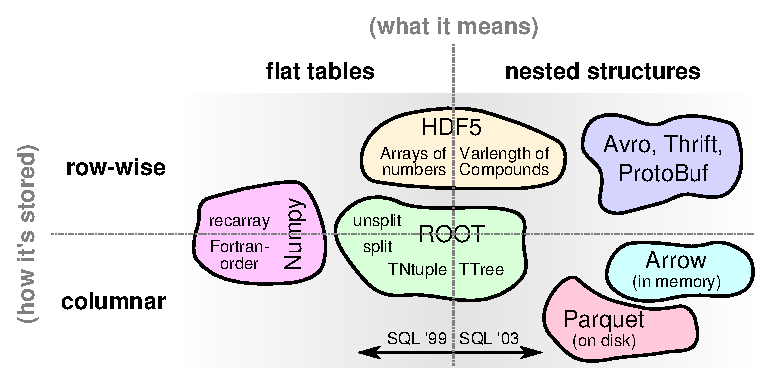
\includegraphics{images/table-of-formats.pdf}
 \caption{Existing data-formats used by ML communities.}\label{fig:data-formats}
\end{figure}

\begin{table}[htbp]
 \caption{This table lists various data formats (rows) and ML tools (columns). The \checkmark\ indicates that there is a native solution, while $\times$ means that the conversion from one data-format to another is straightforward. The following notation has been used to denote the data-formats: \textbf{T} Trees, \textbf{F} flat tables, \textbf{M} sparse matrices, \textbf{R} row-wise arrays, \textbf{C} column-wise arrays \textbf{S} static data structures\newline}
 %
 % Please don't comment in text, use hypothesis instead
 %\textcolor{red}{don't root\_numpy and root\_pandas provide straightforward conversion from root to numpy/hdf5 and thereby input formats to tensorflow, theano, scikit learn, sparkml, torch (which would fill the first row with $\times$)?}
 %
 %\centering
 \begin{tabular}{lcccccccccc}
  \hline
                          & TMVA       & TensorFlow & Theano     & Scikit     & R          & Spark      & VW         & libFM      & RGF        & Torch      \\
                          &            &            &            & Learn      &            & ML         &            &            &            &            \\
  \hline
  \hline
  ROOT [\textbf{T, C}]    & \checkmark &            &            &            &            &            &            &            &            &            \\
  CSV [\textbf{F}]        &            & \checkmark & \checkmark & \checkmark & \checkmark & \checkmark & $\times$   & $\times$   & $\times$   & \checkmark \\
  libSVM [\textbf{M}]     &            &            &            &            &            &            & $\times$   & \checkmark & $\times$   &            \\
  VW [\textbf{M}]         &            &            &            &            &            &            & \checkmark &            &            &            \\
  RGF [\textbf{M}]        &            &            &            &            &            &            &            &            & \checkmark &            \\
  NumPy [\textbf{R}]      &            & \checkmark & \checkmark & \checkmark & \checkmark & \checkmark & $\times$   & $\times$   & $\times$   & \checkmark \\
  Avro [\textbf{S, R}]    &            &            &            &            & \checkmark & \checkmark &            &            &            &            \\
  Parquet [\textbf{S, C}] &            &            &            &            & \checkmark & \checkmark &            &            &            &            \\
  HDF5 [\textbf{S}]       &            & $\times$   & $\times$   & $\times$   &            &            &            &            &            & \checkmark \\
  R df [\textbf{R}]       &            &            &            &            & \checkmark &            &            &            &            &            \\
  \hline
 \end{tabular}\label{tab:formats_vs_tools}
\end{table}
%The de-facto HEP data format is ROOT, used by current HEP experiments and software systems. Although it is very well suited to store and process physics events, it is seldom  used outside of HEP.
\subsubsection{Desirable HEP-ML Software and Data Format Attributes}

A desirable data format should have the following attributes: high read-write speed for efficient training, sparse readability without loading the entire dataset into RAM, compression, and common use by the machine learning community.

HEP machine learning applications require highly performant and flexible algorithms to address the variety of use cases. Some applications, such as triggering, also have to work under tight latency constraints of the order of a few microseconds and below. The data sets are extremely large, which comes with I/O challenges as described in Section~\ref{sec:software_IO}. This is expected to become even more challenging, as the LHC continues to ramp-up and deliver increasingly large amounts of data.

%All of these constitute requirements on ML tools used by the HEP community.
%There are further requirements. The HEP community, for example, is looking to elevate Python to a first class library.
As discussed in Section~\ref{sec:software_proglang}, machine learning tools use a number of languages. To use these tools it will therefore be important to offer adequate support. C++ converters or similar tools are also needed to make sure the training result can be efficiently evaluated.

Advantages of using the {\bf external tools} are the size of the community that uses and supports them, being able to easily keep up with progress in the industry and profit from the forefront of the ML research.
It should also be noted that some of the recent industrial efforts to develop and maintain ML-tools rely on resources far beyond that of basic research. The deep learning tools of the previous and current generations constitute a demonstration of corresponding quality.

Disadvantages of using external tools are that there are too many choices, they are not guaranteed to be supported over the lifetime of particle physics experiments, and it can be difficult to adapt them to HEP specific requirements which may not be among the priorities of the ML community.

Advantages of using {\bf internal tools} are that decisions about long-term support remain in the community, and the tools can be adapted to the specific needs of HEP. Disadvantages include the challenges in incorporating new algorithms and ideas on a timely basis and a possible lack of resources for long-term maintenance.

\subsubsection{Interfaces and Middleware}

One approach to bridge the gap between internal and external tools is by building interfaces. Some researchers prefer to convert their data to the file formats used by external tools and to work exclusively with external tools. This has the advantage of working as close as possible with the ML community's tools and its documentation, and is as close to what is used by ML researchers as possible.
At the same time, interfaces have been built between TMVA and external machine learning tools, allowing for their use and direct comparison between their performance. Currently, interfaces to R, scikit-learn, keras and tensorflow have been developed. Those have the advantage of providing a homogeneous interface and require little training overhead for those already knowledgable in using TMVA.

A more general approach to file format conversion is to build middleware solutions that export HEP-specific formats like ROOT to formats used by external machine learning tools.
%\textit{Caution: this middleware doesn’t imply that it hides completely the other layers. Here one needs knowledge on both inputs and outputs to make a bridge between the HEP tools and external tools.}
%As part of the effort to increase collaboration and bring the HEP community closer to the machine learning community, we foresee that providing a suitable middle-ware solutions to convert ROOT based data to various data-formats is a crucial component to collaboration.
Existing middleware solutions are shown in Table~\ref{table:Middleware}.

Approaches to bridge the different languages and data formats inside and outside of HEP include providing interfaces or building middleware solutions that translate HEP-specific data formats to external ML tools. It is a topic of current research to determine the most efficient solution.

\begin{table}[htbp]
 \caption{Middleware solutions translating the ROOT data format to other formats.}
 \begin{center}
  \begin{tabular}{|l|l|}
   \hline
   \textbf{PyROOT}       & Python extension module that allows the user to interact with ROOT data/classes.~\cite{PyROOT}          \\
   \hline
   \textbf{root\_numpy}  & The interface between ROOT and NumPy supported by the Scikit-HEP community.~\cite{root_numpy}           \\
   \hline
   \textbf{root\_pandas} & The interface between ROOT and Pandas dataframes supported by the DIANA/HEP project.~\cite{root_pandas} \\
   \hline
   \textbf{uproot}       & A high throughput I/O interface between ROOT and NumPy.~\cite{uproot}                                   \\
   \hline
   \textbf{c2numpy}      & Pure C-based code to convert ROOT data into Numpy arrays                                                \\
                         & which can be used in C/C++ frameworks.~\cite{c2numpy}                                                   \\
   \hline

   \textbf{root4j}       & The hep.io.root package contains a simple Java interface for reading ROOT files.                        \\
                         & This tool has been developed based on freehep-rootio.~\cite{root4j}                                     \\
   \hline

   \textbf{root2npy}     & The \texttt{go-hep} package contains a reading ROOT files.                                              \\
                         & This tool has been developed based on freehep-rootio.~\cite{root4j}                                     \\
   \hline

   \textbf{root2hdf5}    & Converts ROOT files containing TTrees into HDF5 files containing HDF5 tables.~\cite{root2hdf5}          \\
   \hline
  \end{tabular}
 \end{center}
 \label{table:Middleware}
\end{table}

%\subsubsection
%The fast paced improvements of external tools and the large number of researchers and practitioners working on them means that it will be almost impossible for the HEP community to keep up with the improvements. As a result, external machine learning tools will be used by HEP physicists to maximize their physics output.


%\paragraph{Conclusion}
%\begin{itemize}
%	\item ROOT might become more modular
%	\item The least risky way: opening HEP to more/many alternatives to ROOT in parallel
%	\item Decide the right level of abstraction to make it adaptable for many languages and tools
%	\item Survey what local solutions have been already implemented with their local experts
%	\begin{itemize}
%		\item get an overview on the trends
%		\item make a database of expertise within the HEP community
%		\item contact HEP people who left for industry and benefit from their double-expertise Let’s bring a couple of people doing that? Relatively easy.
%	\end{itemize}
%	\item Cope with the risk of obsolete %language/tool/package with good archiving methods
%	\item Software development effort is needed in any way
%	\begin{itemize}
%		\item Maintaining HEP internal tools
%		\item Maintaining interfaces between internal and external tools
%		\item Contribution to external tools (for long term support or to provide HEP specific features)
%	\end{itemize}
%\end{itemize}

%\paragraph{Modularisation demands and ideas for ROOT}
%\begin{itemize}
%\item Modular I/O (direct read/write to numpy/hdf5/…)
%\item Modular plotting (e.g. use matplotlib)
%\item Modular machine learning
%\item Modular math (e.g. eigen)
%\end{itemize}
